\chapter{I Linked Open Data in ambito archivistico}

\section{L'eredità culturale: dai graffiti ad oggi}

Tramandare le conoscenze e le esperienze dal vecchio al giovane è un'impresa che ha coinvolto l'uomo fin dal primo segno tracciato sulla parete della caverna che gli dava riparo.\\
L'importanza di lasciare in eredità il sapere accumulato così che chi fosse venuto dopo avesse potuto comprenderlo, rettificarlo e migliorarlo è stata fondamentale durante tutta l'evoluzione culturale dell'uomo, permettendo continue applicazioni, riusi e affinamenti di un corpus enciclopedico sempre più vasto e utile.

In parallelo al miglioramento del sapere in sé è avvenuto un miglioramento dei mezzi per la trasmissione di quest'ultimo, in termini di comprensibilità, durabilità e praticità. Con i racconti omerici e i Vangeli del tutto sensibili a riletture e deformazioni a causa della trasmissione orale, nacquero le immense biblioteche monacensi; la stampa seriale superò il limite della scarsa diffusione e accessibilità di queste ultime. La fotografia e la microfotografia permisero una riproducibilità più rapida ed affidabile, i computer la migliorarono ulteriormente assieme alla risoluzione dei problemi di conservazione.

\subsection{Una rete multiforme}
Ai giorni nostri, le reti di computer (e più nello specifico, Internet) hanno permesso una maggiore pervasività e disponibilità dell'informazione, accessibile ormai a chiunque in tempi pressoché istantanei, per quanto riguarda sia la fruizione sia la creazione di contenuti e conoscenze.\\
Tale velocità e apertura è allo stesso tempo il suo punto di forza e di debolezza: i problemi attuali sono infatti l'autorevolezza (e il conseguente ``rumore digitale'') ma soprattutto la definizione di formati standard comuni per definizione, fruizione e riuso delle informazioni.

\subsection{Il web semantico}\label{sec:semantic-web}
Il potere principale della rete è quello, appunto, di essere una rete, ovvero di poter interconnettere pezzi (\emph{risorse}) di informazione presenti in ``luoghi'' diversi tra di loro e permettere di seguire un percorso in base ai collegamenti propri della risorsa che stiamo esaminando, fin dalla prima formulazione dello standard HTML.\\
Oggi assistiamo ad una evoluzione (fig.~\ref{fig:web_evolution}) del modo di fruire la rete nell'interconnessione non solo dei documenti, ai quali era inizialmente limitato il web, ma anche degli utenti (Web 2.0); tale evoluzione sta procedendo nella direzione del \emph{web semantico}, dove tutto (documenti, utenti, concetti, persone, etc.) è considerato una \emph{risorsa} ed è collegato e collegabile con altre risorse, idealmente racchiudendo tramite tale struttura a grafo tutta l'informazione umana (Web 3.0\footnote{Il nome \emph{Web 3.0} è stato usato inizialmente da Jeffrey Zeldman \cite{30} e quindi ripreso da Tim Berners-Lee \cite{31} in riferimento ad un web più ``intelligente'' che comprenda, oltre all'informazione aperta e strutturata, anche connessione onnipresente, formati aperti, dati nella nuvola e più in generale l'abbandono del legame alla ``fisicità'' degli strumenti per l'accesso alla rete stessa}).

\begin{figure}[ht!]
	\centering
	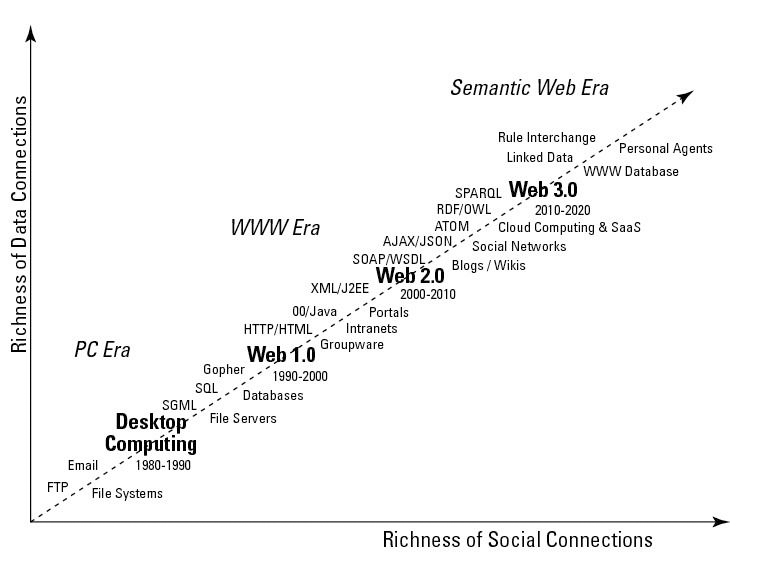
\includegraphics[width=90mm]{images/Four-major-waves-of-Web-evolution.jpg}
	\caption{Evoluzione del web, in \cite{1}}
	\label{fig:web_evolution}
\end{figure}

Il web semantico si concentra quindi:
\begin{quote}
sui dati e sul formato di rappresentazione degli stessi, sul linguaggio e su come i dati si relazionano agli oggetti del mondo reale, il che permette ad una persona o ad una macchina di seguire un percorso tra dati di natura diversa che non sia attraverso dei cavi bensì tramite collegamenti semantici.\cite{2}
\end{quote}

\subsection{Giant Global Graph e Linked Open Data}
Questo spostamento d'accento dal documento in sé alla relazione che intercorre con altre risorse è stato sottolineato da Tim Berners-Lee (co-inventore del World Wide Web) nel suo articolo \emph{Giant Global Graph} \cite{3}, evidenziando come il salire sopra al livello del singolo documento permetta il riuso dell'informazione\footnote{\url{https://www.youtube.com/watch?v=OM6XIICm_qo}}.

Il concetto di \emph{Linked Open Data} (LOD) implementa il web semantico permettendo la creazione di relazioni (\emph{link}) tra risorse (\emph{data}) e rendendole fruibili e accessibili (\emph{open}) così da favorirne e incoraggiarne l'uso e il riuso.

Berners-Lee concettualizza i LOD definendo quattro regole:
\begin{enumerate}
\item Usate gli URI come nome per le cose.
\item Usate URI HTTP così che gli utenti possano recuperarli.
\item Quando un utente accede ad un URI fornite informazioni utili attraverso gli standard (RDF, SPARQL).
\item Includete collegamenti ad altri URI così che gli utenti possano scoprire più cose.
\end{enumerate}
Se una sola di queste regole è disattesa, secondo Berners-Lee non si può parlare di LOD. \cite{4}

La rappresentazione dei dati, dovendo essere comprensibile tanto all'uomo quando alla macchina, si è fatta forte del costrutto più basilare del linguaggio, ovvero la struttura \verb"soggetto-predicato-oggetto": lo standard per i LOD è infatti RDF\footnote{\url{http://it.wikipedia.org/wiki/Resource_Description_Framework}}, dove ogni relazione viene rappresentata per l'appunto da una tale tripla (chiamata \emph{statement}).\\
Ad esempio, nello statement \texttt{Federico Zeri è autore della fotografia \#231} abbiamo
\begin{itemize}
\item \verb"Federico Zeri" come soggetto
\item \verb"è autore di" come predicato
\item \verb"fotografia #231" come oggetto
\end{itemize}
Questa formulazione non fa assunzioni sul dominio del discorso e lascia pertanto completa libertà sulla formulazione degli statement che risultano comprensibili tanto dall'uomo quanto dalla macchina.

\section{I LOD per l'eredità culturale}

L'avvento dei LOD ha aperto un interessante campo di studio e ricerca in particolare per biblioteche, archivi e musei, costantemente alla ricerca  e alla sperimentazione di nuovi modi per rendere i dati disponibili, fruibili e riusabili dagli utenti \cite{5}. Lo sforzo da parte di queste istituzioni è sempre stato quello di conservare e migliorare la visione e revisione dei contenuti da parte di studiosi, ricercatori e utenti in genere; è quindi naturale che la possibilità di intercorrelare le informazioni diventi particolarmente appetibile.

\subsection{LOD e archivi}
L'introduzione di una nuova pratica o tecnologia comporta un normale periodo di ``rodaggio'' iniziale, spesso accompagnato da una frammentazione durante la definizione di uno o più standard da seguire.\\
Sebbene la curva di crescita dei LOD appaia decisamente ripida (fig.~\ref{fig:lod-cloud}) come evidenzia \cite{21}, coinvolgendo alcune delle più importanti organizzazioni a livello mondiale, moltissimi archivi ne restano ancora esclusi, principalmente per la mancanza di mezzi economici e tecnologici che riescano a convertire i database, pur dettagliati e articolati, in dataset aperti aderenti agli standard che caratterizzano la nuvola dei LOD.

\begin{figure}
    \centering
    \begin{subfigure}[b]{0.5\textwidth}
            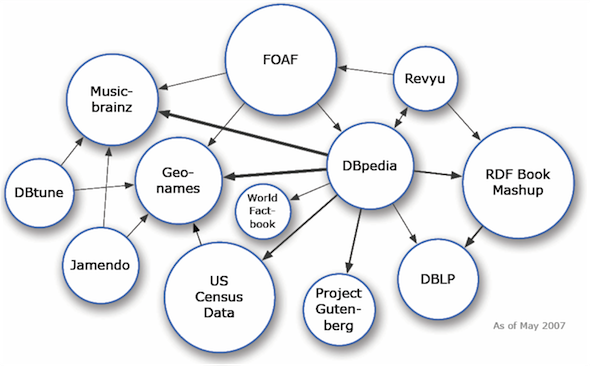
\includegraphics[width=\textwidth]{images/lod-cloud-2007.png}
            \caption{Maggio 2007}
            \label{fig:lod-cloud-2007}
    \end{subfigure}%
    ~ %add desired spacing between images, e. g. ~, \quad, \qquad, \hfill etc.
      %(or a blank line to force the subfigure onto a new line)
    \begin{subfigure}[b]{0.5\textwidth}
            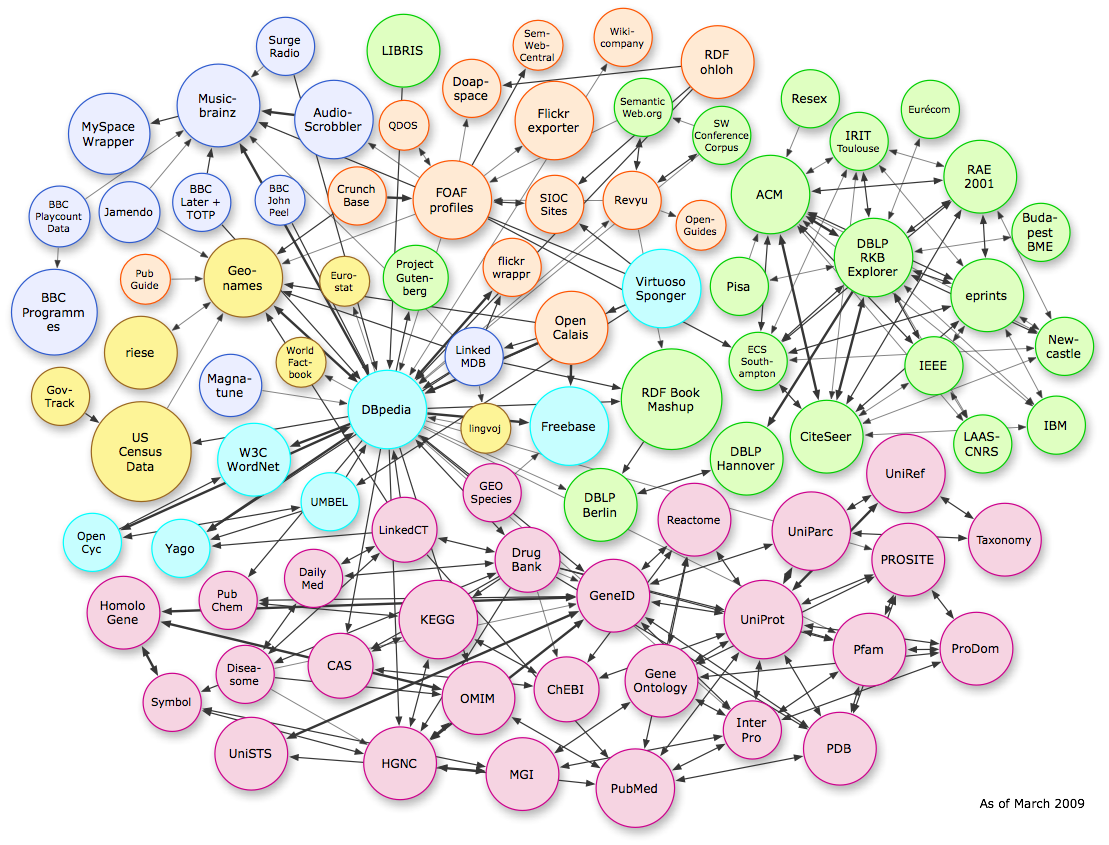
\includegraphics[width=\textwidth]{images/lod-cloud-2009.png}
            \caption{Marzo 2009}
            \label{fig:lod-cloud-2009}
    \end{subfigure}
    %add desired spacing between images, e. g. ~, \quad, \qquad, \hfill etc.
    %(or a blank line to force the subfigure onto a new line)

    \begin{subfigure}[b]{\textwidth}
            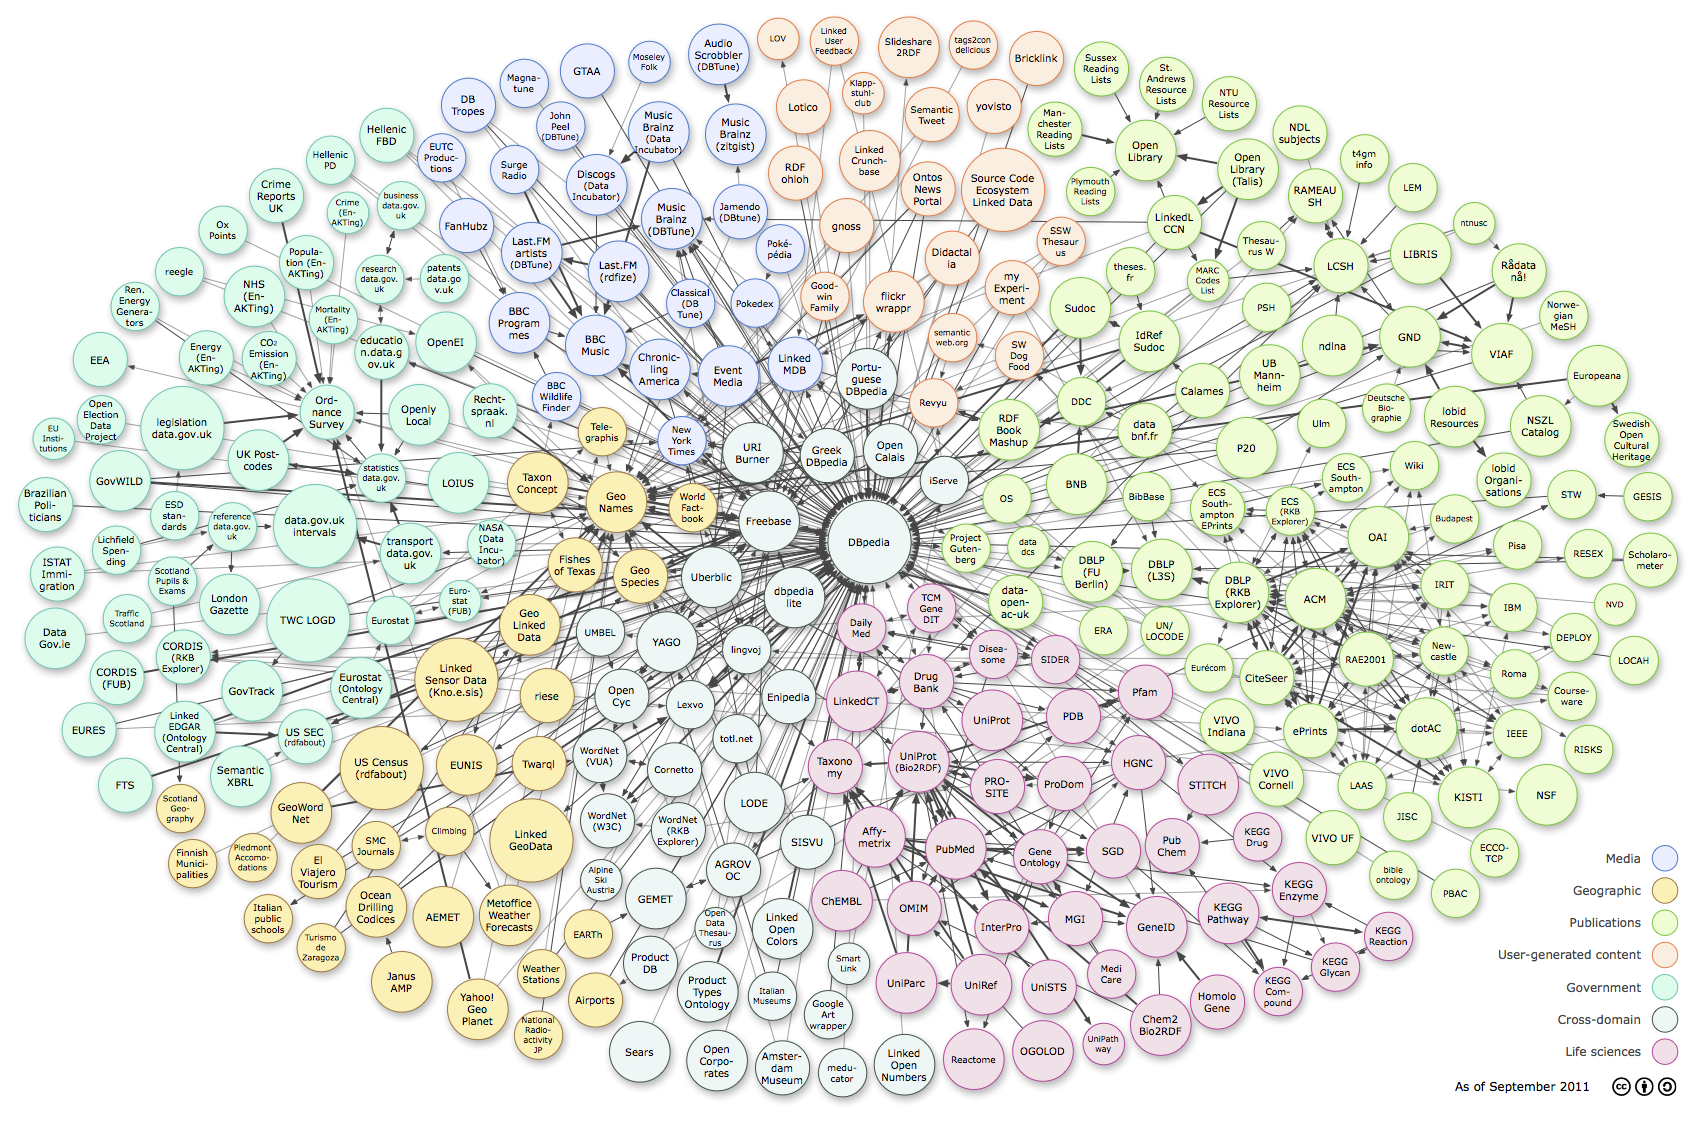
\includegraphics[width=\textwidth]{images/lod-cloud-2011.png}
            \caption{Situazione attuale}
            \label{fig:lod-cloud-2011}
    \end{subfigure}
    \caption{Evoluzione dei dataset pubblicati in LOD (fonte: \protect\url{http://lod-cloud.net})}
    \label{fig:lod-cloud}
\end{figure}

All'intrinseca difficoltà tecnologica propria di qualsiasi conversione di un dataset da un formato ad un altro, si aggiunge la difficoltà della mancata neutralità culturale dei dati che comporta quindi la necessità di effettuare delle precise scelte riguardo il modello descrittivo dei dati (ovvero i metadati che li descrivono) e riguardo il modello concettuale degli stessi, ovvero le ontologie scelte per la conversione.

Quest'ultima scelta diventa ancora più critica in rapporto alla quantità ed eterogeneità degli standard esistenti e attualmente adottati dalle principali entità che si occupano della preservazione dei dati culturali \cite{6}; la mappatura delle ontologie nel dominio LOD (e.g. \cite{7}) è perciò un argomento che sta particolarmente a cuore non solo da un punto di vista tecnico ma anche e soprattutto da un punto di vista concettuale: progetti come \emph{Europeana}\footnote{\url{http://www.europeana.eu}} ne fanno un centrale argomento di discussione.

\newpage
\subsubsection{L'approccio concettuale}

\begin{wrapfigure}{r}{0.4\textwidth}
  \vspace{-20pt}
  \begin{center}
    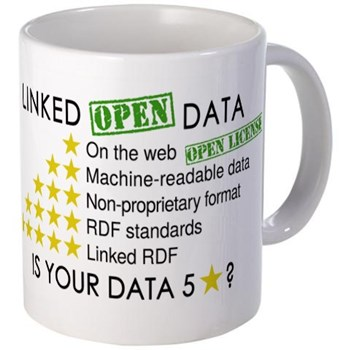
\includegraphics[width=0.4\textwidth]{images/5_star_linked_open_data_mug.jpg}
  \end{center}
  \vspace{-20pt}
  \caption{I vostri LOD sono a 5 stelle? \cite{4}}
  \vspace{-10pt}
\end{wrapfigure}

Prima di pensare all'indispensabile automazione, dal momento che convertire manualmente gli enormi database attualmente in essere sarebbe umanamente impossibile, è necessaria una chiara comprensione di ciò che attualmente esiste per potersene avvantaggiare in maniera proficua.

Tornando alla concettualizzazione di Berners-Lee vista poc'anzi \cite{4}, l'autore aggiunge (nel 2010) un sistema a 5 stelle per definire la qualità dei LOD:
\begin{description}
\item[1 stella] I dati sono sul web in un qualsiasi formato ma \emph{con licenza aperta}.
\item[2 stelle] Come sopra e in più leggibili da una macchina (e.g. una tabella Excel al posto di una scansione della stessa tabella)
\item[3 stelle] Come sopra ma in formato non proprietario (e.g. CSV invece che Excel)
\item[4 stelle] Come sopra ma usano standard del W3C (RDF e SPARQL) per identificare le risorse così da permetterne il collegamento da parte degli utenti
\item[5 stelle] Come sopra e inoltre sono collegati a dati di altre entità.
\end{description}

Questa classificazione si scontra naturalmente con la realtà di fatto: molte istituzioni non sono ancora pronte per il sistema di Berners-Lee perché i dati sono collegati ma non aperti o perché i dataset sono aperti ma debolmente collegati \cite{5}.

Diventa quindi fondamentale la formulazione di un approccio che tenga conto degli sviluppi futuri, attraverso precise metodologie del web semantico e strumenti adeguati, per trarre vantaggio il più possibile dalla ricchezza degli archivi stessi: la formulazione di un processo di conversione è di importanza vitale per garantire la persistenza del dettaglio dei dati di partenza e l'aderenza dei dati di arrivo a degli standard che garantiscano un più che buon livello di interoperabilità. I due approcci possibili in un tale progetto di conversione sono diametralmente opposti.

Il primo mira ad esportare l'intero dataset considerando ogni record come entità ontologica unica e atomica, ottenendo quindi una rappresentazione diretta e appiattita dell'archivio dati. Questa metodologia consente di ottenere velocemente un risultato consistente con la base dati, inscatolando la complessità e l'eventuale divergenza con gli standard all'interno di un'entità che viene gestita come elemento unitario. Collassare gli strati di informazione è pure rischioso per il successivo recupero e riuso dei singoli elementi contenuti nel record, come evidenziato da \cite{8}.

Il secondo prevede un'analisi più complessa e profonda che porti alla divisione di ogni record in elementi atomici intercorrelati riportati su uno strato di astrazione; in questo modo si ottiene un grafo concettuale riusabile e aderente al sistema a 5 stelle di Berners-Lee, al costo di un maggior dispendio di energie nel lavoro di analisi, conversione e revisione dei dati.

\section{Un caso concreto: Zeri e LODE}
Come modello concreto per la conversione di un archivio in LOD è stato considerato l'archivio fotografico della Fondazione Zeri, un'estesa collezione di fotografie di dipinti catalogate in un RDBMS tradizionale con l'obiettivo di esportarle nel dominio LOD adottando CIDOC-CRM come modello descrittivo e concettuale.

Il progetto è stato battezzato \emph{Zeri e LODE}\footnote{da LODE - Live OWL Documentation Environment, \url{http://www.essepuntato.it/lode}}.

\subsection{L'archivio fotografico Zeri}
La collezione fotografica lasciata da Federico Zeri (1921-1998) all'Università di Bologna è un corpus di 290.000 immagini di opere d'arte e monumenti dettagliatamente catalogate e organizzate dal ricercatore lungo tutta la sua carriera\footnote{\url{http://www.fondazionezeri.unibo.it/home/fototeca/00000045_la_fototeca.html}}.\\
La rarità del materiale e della documentazione raccolta nella collezione ne fa un'importantissima fonte di informazione, al punto da venir definita come

\begin{quote}
The first, and no doubt the most important database on art history.\hspace*{\fill}(The Art Tribune, 16 agosto 2010)
\end{quote}

L'archivio è, infatti, prezioso non solo per la rarità e qualità del materiale contenuto, ma soprattutto per il meticoloso lavoro di descrizione storica eseguito da Zeri, che credeva nella fotografia come strumento fondamentale per lo studio e l'analisi filologica delle opere d'arte. Il potere descrittivo e analitico della fotografia in bianco e nero applicato ad un occhio sensibile permetteva di notare sottili variazioni di colore e trama delle opere, paradossalmente meno evidenti in fotografie a colori.

Zeri ha sempre lavorato in modo da costituire un archivio che potesse essere aperto e reso fruibile a chiunque per ricerche, studi e sviluppi; proseguendo gli sforzi del ricercatore, la Fondazione Federico Zeri si è impegnata fin dalla sua costituzione (2002) per rendere accessibile l'archivio fotografico a ricercatori e studenti attraverso la digitalizzazione e catalogazione dell'intera collezione.

\subsection{Il database e la scheda F}
Il risultato del lavoro della Fondazione è un database pubblicamente accessibile in \url{http://www.fondazionezeri.unibo.it} che al momento conta circa 160.000 delle 290.000 fotografie della collezione, consultato da più di 70.000 utenti unici nel solo 2013.

Per ottenenere tale risultato il lavoro di catalogazione è stato preceduto da un'intensa fase analitica: la destinazione d'uso di un simile catalogo richiedeva l'utilizzo di una struttura compatibile con gli standard catalografici italiani definiti dal Ministero per i Beni Culturali\footnote{\url{http://www.iccd.beniculturali.it}} che pure fosse sufficientemente articolata per mantenere la specificità della collezione come organizzata da Federico Zeri.

\begin{figure}[p!]
    \centering
    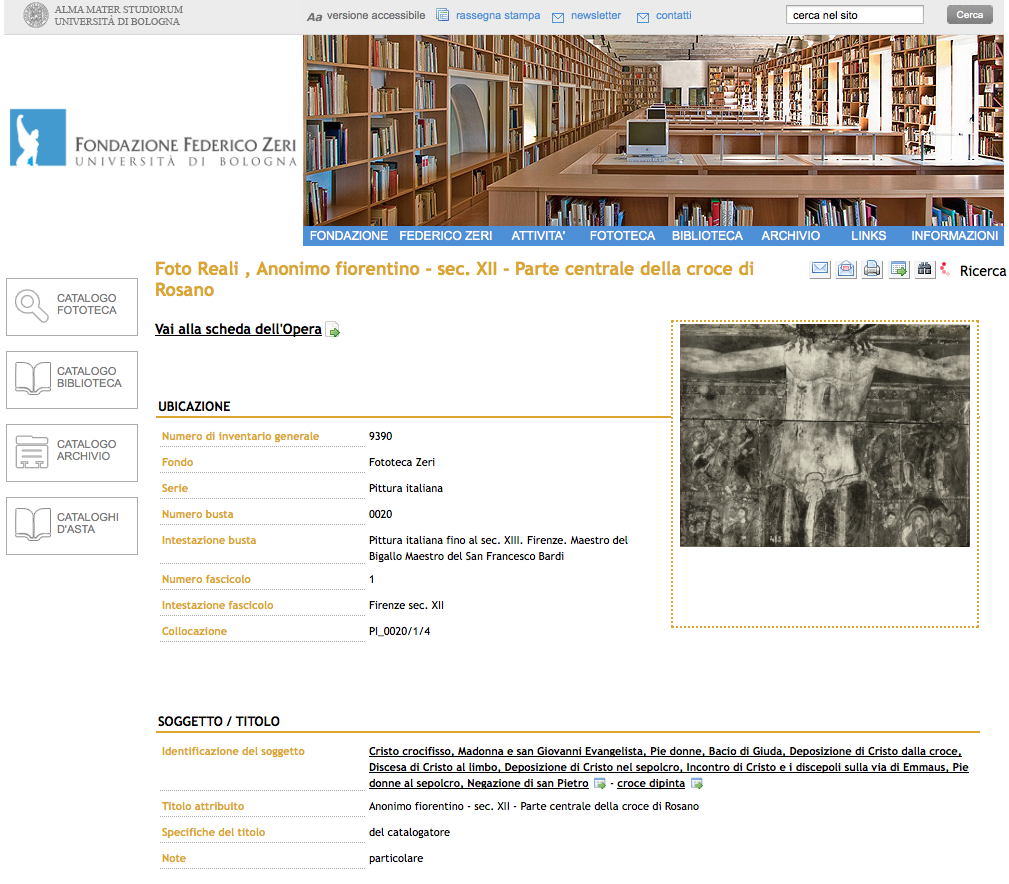
\includegraphics[width=\textwidth]{images/fondazionezeri-screen.png}
	\caption{Esempio di scheda F (fonte: \protect\url{http://www.fondazionezeri.unibo.it/catalogo/})}
	\label{fig:fondazionezeri-screen}
\end{figure}

La scelta del modello descrittivo e concettuale da seguire è ricaduta in modo naturale sulla \emph{Scheda F}\footnote{\url{http://www.iccd.beniculturali.it/index.php?it/387/beni-fotografici}} (dove \emph{F} sta per \emph{Fotografia}) proposto dall'Istituto Centrale per il Catalogo e la Documentazione (ICCD) nella sua versione 3.0.\\
Lo standard \emph{Scheda F} fu accettato solo nel 1999 dopo un intenso dibattito concluso con il riconoscimento, sancito dal ``Testo Unico delle disposizioni legislative in materia di Beni Culturali e Ambientali'' (\cite{16}), della fotografia come bene culturale disciplinato (art 2, comma 2), innalzandola in dignità dal ruolo di pura funzione documentaria che le era stato fino a quel momento attribuito.\\
Nonostante l'iniziale difficoltà di accettazione di questo nuovo standard, causate principalmente dal dettaglio dei campi e la complessità delle norme catalografiche, la validità scientifica della Scheda F è riconosciuta e innegabile, portando nel 2004 ad una revisione (v. 3.00) e attualmente ad una sperimentazione più approfondita con la possibilità di descrivere set complessi oltre a elementi individuali (v. 4.00).\\
Tra i database disponibili sul Web che adottano la Scheda F si possono evidenziare il \emph{SIRPAC - Sistema Informativo Regionale del Patrimonio Culturale del Friuli-Venezia Giulia}\footnote{\url{http://www.sirpac-fvg.org/}}, il portale \emph{Lombardia Beni Culturali}\footnote{\url{http://www.lombardiabeniculturali.it/fotografie/}}, il catalogo \emph{Guarini Patrimonio Culturale}\footnote{\url{http://www.regione.piemonte.it/cultura/GPCWeb/zf/}}, il portale \emph{Beni Culturali Veneto}\footnote{\url{http://catalogo.regione.veneto.it/beniculturali/}}, \emph{L'album di Roma: Fotografie private del Novecento}\footnote{\url{http://www.albumdiroma.it/sicap/opac.aspx?Web=ROMA}}; tali database si avvantaggiano del sistema SIGECweb\footnote{\url{http://www.iccd.beniculturali.it/index.php?it/118/sistema-informativo-generale-del-catalogo-sigec}} attualmente in sviluppo da parte dell'ICCD e in futuro consultabile online.

La complessità e il dettaglio della Scheda F sono allo stesso tempo il maggior punto di forza e di debolezza del modello: le strette norme di catalogazione ne hanno in qualche modo scoraggiato l'adozione per lungo tempo, pure i principi sui quali si basa sono attuali e proiettati verso il riconoscimento degli archivi fotografici come bene con dignità autonoma e non più come documentazione delle opere d'arte fotografate.

Diverse istituzioni si stanno muovendo in questa direzione (e.g. la Berenson Library\footnote{\url{http://itatti.harvard.edu/berenson-library/collections/fototeca-photograph-archive}}, parte della Harvard University, alcuni archivi tedeschi (Hertziana, Kunst Historisches Institute of Florence) parte del Bildarchiv Photo Marburg\footnote{\url{http://www.fotomarburg.de/}}); pure l'attuale interesse all'oggetto fotografico in alcuni casi non è garanzia di precisione nella catalogazione dell'oggetto reale (come avviene, ad esempio, in \emph{Europeana} \cite{8}).

Questo avviene proprio a causa del fisiologico grado di personalizzazione degli standard applicato dalle singole istituzioni per accomodare la specificità dell'archivio catalografico pregresso, spesso sfruttando un ridotto sottoinsieme dei campi messi a disposizione e creando campi fuori standard per conservare dati che altrimenti andrebbero perduti.

Tornando in particolare all'archivio di Zeri, la quantità e particolarità di informazioni registrate sul retro o a margine delle fotografie dallo studioso ha reso necessaria un'espansione e adattamento del modello in essere: degli oltre 300 campi presenti nella versione estesa, la Fondazione Zeri ne ha adottati 113 organizzati in blocchi (definiti \emph{paragrafi}) e aggiungendone alcuni specifici, in parte adottati nello sviluppo della versione 4.0 del modello ministeriale.

I paragrafi replicano l'organizzazione dei dati sulla carta: autore della fotografia, soggetto, titolo, indicazioni cronologiche riguardo lo scatto, movimenti e acquisizioni, dati tecnici, stato di conservazione, copyright e codici identificativi.

Data la natura del soggetto ritratto (opera d'arte) la catalogazione non poteva prescindere dalla raccolta e conservazione delle informazioni a riguardo; è stato quindi affiancato un secondo modello per la descrizione delle opere ritratte, nella fattispecie la \emph{Scheda OA}\footnote{\url{http://www.iccd.beniculturali.it/index.php?it/253/beni-storici-e-artistici}} (dove \emph{OA} sta per \emph{Opera d'Arte}) di ICCD. Qui viene descritto il contenuto semantico della fotografia attraverso altri 79 campi che offrono una dettagliata descrizione riguardo tipo, soggetto, attribuzioni, cronologia, movimenti, materiali, tecniche e riferimenti bibliografici.

Tali informazioni sono principalmente dedotte dalle annotazioni di Zeri sul retro delle fotografie, dalla documentazione che le accompagna e dai volumi presenti nella sua biblioteca.

Ogni Scheda OA è collegata all'insieme delle schede F che ritraggono l'opera; queste ultime sono a loro volta collegate alle relative rappresentazioni digitali (alta e bassa risoluzione, miniatura e scansione del retro della fotografia).

La presenza di due modelli distinti e paralleli permette di fatto la creazione di due cataloghi distinti e correlati, l'uno di materiale fotografico e l'altro di opere d'arte, rendendo quindi possibile una ricerca e navigazione trasversale da parte degli utenti.

I due cataloghi si avvantaggiano di sei \emph{Authority File} (ovvero cataloghi che mirano ad unificare i riferimenti ad entità esterne quali autori, soggetti, bibliografie, etc\ldots\footnote{\url{http://en.wikipedia.org/wiki/Authority_control}}) che forniscono dataset particolareggiati riguardo fotografi, collezioni, artisti, bibliografie, cataloghi d'asta e documenti associati, alcuni di questi accessibili online come database autonomi.

L'indice attuale include, oltre alle fotografie, documenti e cataloghi d'asta, tutti nello stesso contesto; ogni elemento è catalogato e collegato alla scheda dell'opera dal quale deriva, facendo di quest'ultima di fatto il nucleo centrale attorno al quale si dipana tutta la ricerca di Federico Zeri: fotografie, libri e documenti cartacei.

\subsection{Verso un nuovo modello: CIDOC-CRM}\label{sec:towards-a-new-model}
Al momento attuale il database dell'archivio Zeri arriva già a 3 stelle nel sistema di Berners-Lee: è infatti sul web\footnote{\url{http://www.fondazionezeri.unibo.it/catalogo}} con licenza aperta, in formato automatizzabile (\emph{XML}) e standard (\emph{ICCD - Scheda F}). Tali caratteristiche hanno permesso alla Fondazione Zeri di contribuire in maniera significativa a progetti internazionali e portali quali \emph{Europeana}\footnote{\url{http://europeana.eu/}} e \emph{Artstor}\footnote{\url{http://www.artstor.org/}}.

Con l'accrescimento del corpus catalografico e delle esigenze di consultazione e di interscambio con altri cataloghi nasce l'esigenza di esportare i dati in modo più strutturato e in linea con gli standard dei LOD, similarmente a quanto già fatto da altre istituzioni (e.g. \cite{5,9,10,11,12}), il cui lavoro si concentra principalmente sulla conversione del database, la creazione del triple store, il collegamento nel dominio LOD e la realizzazione dell'interfaccia di navigazione.

Nel gennaio del 2013, durante un meeting di due giorni a New York dedicato alle prospettive future per gli archivi della documentazione storico-artistica, è nato il gruppo \emph{International Digital Photo Archive Consortium} (IDPAC), del quale fanno parte, oltre alla Fondazione Federico Zeri, altre tredici istituzioni\footnote{\url{http://www.frick.org/photoarchive/discoveries/future_photoarchives\#sthash.pIMY0SfV.dpuf}} con un archivio totale di 31 milioni di foto di opere d'arte.

Uno degli scopi del gruppo è discutere e verificare la possibilià di creare una piattaforma comune per la condivisione delle rispettive risorse digitali e di collegare i dati per facilitarne l'accesso, in modo da realizzare una vera e popria banca dati globale per la ricerca storica d'arte.

Seppure ancora in fase di esplorazione, il gruppo ha identificato CIDOC-CRM \cite{13} come ontologia più adatta e adattabile a mappare i dati provenienti da molteplici fonti disgiunte, per la sua focalizzazione nel rappresentare la maggior parte degli standard dell'eredità culturale.

Forte di tali esperienze già in essere, il metodo di mappatura è stato focalizzato proprio attorno a CIDOC-CRM, che effettivamente rappresenta la tecnologia più utilizzata nel campo dell'eredità culturale\footnote{\url{http://www.cidoc-crm.org/uses_applications.html}} e permette una concettualizzazione semantica del materiale fotografico in un'ottica FRBR, già ampiamente in uso sebbene talvolta non nel modo adeguato, data la sua natura di dominio bibliografico promosso solo in un secondo momento a framework concettuale.

Inoltre è innegabile l'apporto di altri modelli di produzione di LOD per l'eredità culturale, quali la Library of Congress\footnote{\url{http://id.loc.gov}}, VIAF\footnote{\url{http://viaf.org/}}, CulturaItalia\footnote{\url{http://dati.culturaitalia.it/}}, Bibliothèque nationale de France\footnote{\url{http://data.bnf.fr}}, Deutsche National Bibliothek\footnote{\url{http://www.dnb.de/EN/lds}}, Archives HUB\footnote{\url{http://datahub.io/dataset/archiveshub-linkeddata}}.\\
Tesauri come il \emph{Getty Art \& Architecture Thesaurus®}\footnote{\url{http://www.getty.edu/research/tools/vocabularies/aat/}} e \emph{Iconclass}\footnote{\url{http://www.iconclass.nl/}} sono altresì importanti fonti di dati; anche il \emph{Nuovo Soggettario della Biblioteca Nazionale Centrale Firenze}\footnote{\url{http://thes.bncf.firenze.sbn.it/thes-dati.htm}} offre l'intero tesauro in formato SKOS/RDF, purtuttavia non essendo ancora in LOD.

Considerando infine il modello EDM (\cite{11}) e le linee guida di mappatura di Europeana\footnote{\url{http://www.iconclass.nl/about-iconclass/what-is-iconclass}}, all'interno del quale il catalogo Zeri è già contenuto, lo sforzo è stato quello di definire un modello proprio per il particolare caso dell'archivio, focalizzandosi sulla separazione semantica secondo FRBR e sfruttando altre ontologie (PROV-O\footnote{\url{http://www.w3.org/TR/prov-o/}} e FaBiO\footnote{\url{http://purl.org/spar/fabio}}) non ancora conosciute nel dominio dell'eredità culturale.

\subsection{CIDOC-CRM e FRBR}

\subsubsection{CIDOC Conceptual Reference Model}
Il CIDOC Conceptual Reference Model (CRM)\footnote{\url{http://cidoc-crm.org}} è un modello nato per offrire una struttura formale a supporto della descrizione in concetti e relazioni utilizzati nel campo dell'eredità culturale. Il framework è pensato per essere sufficientemente generico per essere utilizzato in tutta una serie di ambiti culturali quali musei, biblioteche, archivi, etc\dots ovvero per permettere la mappatura di qualsiasi informazione riguardante l'eredità culturale, in modo da risultare una sorta di ``colla semantica'' tra diverse sorgenti di dati con formati diversi.

CIDOC-CRM è il punto d'arrivo di un lavoro di oltre 10 anni fatto dai gruppi \emph{CIDOC Documentation Standards Working Group} e \emph{CIDOC CRM SIG}, accettato come standard ISO (21127:2006\footnote{\url{http://www.iso.org/iso/catalogue_detail?csnumber=34424}}) dal dicembre del 2006.

\subsubsection{Functional Requirements for Bibliographic Records}

La sigla \emph{FRBR} sta per \emph{Functional Requirements for Bibliographic Records} e indica uno schema concettuale disegnato dall'emph{International Federation of Library Associations} (IFLA\footnote{\url{http://www.ifla.org}} nato in ambito bibliografico per la rappresentazione e la classificazione delle informazioni secondo una struttura a livelli \cite{19}.

Attraverso FRBR la catalogazione ``scompone'' il record bibliografico in quattro livelli fondamentali (fig.~\ref{fig:frbf-levels}:
\begin{description}
\item[Work] l'opera di ingegno concettualmente intesa (e.g. \emph{Alice's Adventures in Wonderland} di Lewis Carroll)
\item[Expression] l'espressione, ovvero la realizzazione concettuale di tale opera (e.g. la traduzione italiana \emph{Le avventure di Alice nel Paese delle Meraviglie})
\item[Manifestation] la realizzazione materiale di una Expression (e.g. l'audiolibro \emph{Alice nel Paese delle Meraviglie})
\item[Item] il singolo esemplare di una Manifestation (e.g. la copia del CD \emph{di Fabio} che contiene l'audiolibro \emph{Alice nel Paese delle Meraviglie})
\end{description}

\begin{figure}
  \centering
  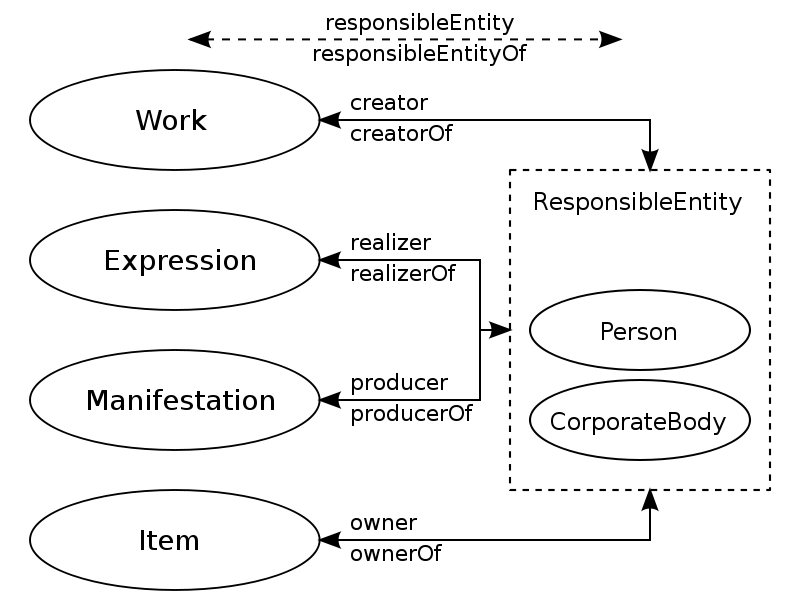
\includegraphics[width=\textwidth]{images/FRBR-Group-2-entities-and-relations.png}
  \caption{I quattro livelli di FRBR e le relazioni con le entità del gruppo 2}\label{fig:frbf-levels}
\end{figure}

Tale suddivisione permette di identificare con precisione il record e unificare i collegamenti in modo concettualmente logico: ad esempio, l'autore viene legato al livello \emph{Work}, l'editore al livello \emph{Manifestation}, il traduttore al livello \emph{Expression} e il possessore al livello \emph{Item} (tali tipologie di entità sono identificate come ``entità del gruppo 2'').

\subsubsection{FRBRoo}

Il naturale punto d'incontro per CIDOC-CRM e FRBR è \emph{FRBRoo}\footnote{\url{http://cidoc-crm.org/frbr_inro.html}}, un'ontologia nata sul modello di CIDOC-CRM per rappresentare la struttura di FRBR in modo che i due modelli possano essere sfruttati insieme.

La prima bozza di FRBRoo è stata pubblicata nel 2006 come modello logicamente rigido che interpreta le concettualizzazioni e le relazioni espresse da FRBR come estensione di CIDOC-CRM.

FRBRoo è arrivato alla sua versione 0.9 nel gennaio del 2008 e approvato dall'IFLA FRBR Review Group nell'agosto del 2008.
